\chapter{Realisierung}

\section{Systemübersicht}

\begin{figure}[H]
	\centering
	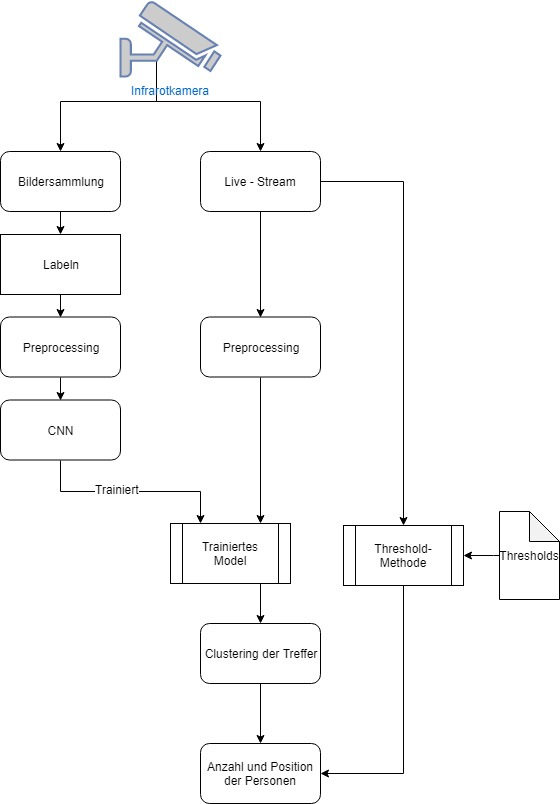
\includegraphics[width=.8\linewidth]{SystemOverview}
	\caption{Grobübersicht des Systems mit CNN- und Thresholdalgorithmus}
	\label{SystemOverview}
\end{figure}

\section{UDP-Schnittstelle}

Um die Bilder automatisiert erhalten zu können wurde eine Schnittstelle zu den Infrarotkameras implementiert. Es wurde das UDP-Protokoll verwendet, da die Kameras nur über dieses Protokoll angesprochen werden konnten.\\
 Die einzige ander Möglichkeit and Bilder zu gelangen wäre über die GUI Applikation des Herstellers Videos aufzunehmen. Dies sind bereits auf RGB convertiert, beihalten also nicht alle Information des ursprünglichen Bildes und die Applikation kann nicht automatisiert angesprochen werden. Folglich ist dies keine praktikable Variante um effizient Daten zu sammeln.\\
\\
Die Kameras können ausserdem nur mittels UDP-Broadcasts identifiziert und 

\subsection{Interne Schnittstellen}


\subsection{Umsetzung Programmierung}

\subsection{Testing}
